\documentclass[11pt]{article} % letterpaper is american!

\usepackage[british,UKenglish,USenglish,english,american]{babel}
\usepackage[pdftex]{graphicx}
\usepackage{epstopdf}

\usepackage{amsfonts,amsmath,amsthm,amssymb}

\usepackage{tikz,pgf}
\usetikzlibrary{fit}

\pagestyle{empty}
\setlength{\parindent}{0mm}
\usepackage[letterpaper, margin=0.5in]{geometry}
%\usepackage{showframe}

\usepackage{multicol}
\usepackage{enumerate}

\usepackage{color}
\usepackage{verbatim}
\usepackage{listings}
\lstset{
  basicstyle=\scriptsize\ttfamily,
  backgroundcolor=\color{lightgray},
  language=bash,
  frame=L,
}


\usepackage{xspace}
\usepackage{url}
\usepackage{cite}

\usepackage{titlesec}
\titlespacing*{\subsubsection}{0pt}{*0}{*0}
\titlespacing*{\subsection}{0pt}{0pt}{*0}
\titlespacing*{\section}{0pt}{0pt}{*0}

\newcommand{\Bold}{\mathbf}


\setlength{\parskip}{1em}
\setlength{\parindent}{1em}

\def\ptk{peval-toolkit\xspace}
\def\ppaml{PPAML\xspace}

\title{New Documentation for PPAML-Eval-Tools}

\date{\today}

\author{Philip Robinson}

\begin{document}
  \maketitle

  \section*{Goals and Requirements}

  It is our goal to provide a \ptk that allows for us to human-efficiently compute and store quantitative metrics for team submissions to the \ppaml program. In this most recent submissions iteration, there was a significant amount of time that lost to setup, configuration, and queueing executions of challenge problem solutions. 

    We have been asked by the teams to provide a more rigid acceptance criteria
  
\newpage
  \section*{Workflow}
  By better discussing the intended worakflow we can outline the changes that need to be applied to the present \ptk.

  \subsection*{Terminal}
  
  \begin{multicols}{2}
  \subsubsection*{Present}
  The ini files beeing addressed/created do not correctly allow for seperation of PPS and CPS. Many of the submissions were delivered such that seperation of the PPS from CPS is not possible. This prevents us from performing progress comparisons. 

  There were also no tools for quereying the database for valid input variables, so teams must know their id values without help (or by using sql queries).

  % We do not presently enfource any restrictions on time or memory usage. 
  
  The present model could be extended to have a cps.ini, pps.ini, and eval.ini files. but this becomes unmanagable quickly, it may be better to have conf.ini that is updated as states are accomplished.  

  % We do not have a trivial way of tagging 
  We need to include reporting tools, database updating/merging, and sample data in the released versions of the \ptk.
  
  \begin{lstlisting}
# create ini file to manually populate only
#   cooresponds to cp-solutions
$ ppaml init <team-id> <challenge-id> 

# run solution as defined by ini file
$ ppaml run <cps.ini>

# evaluate output from run execution
$ ppaml eval <cps.ini>

# reports are externally executed and directly 
#   querey the database
$ ./generate_reports.py 
  \end{lstlisting}
  
  \vfill\columnbreak
  \subsubsection*{Goal}
  Instead of 'team' owning 'pps-type' owning 'pps-instances' it makes sense to just make 'team' representative of pps-type which owns engines\footnote{To increase clarity, I am decoupling the term 'pps' and 'engine'.}
  \begin{lstlisting}
# provide list operations
$ ppaml list teams
$ ppaml list problems

# engines listed by date and population
$ ppaml list engines <team-id> 
  \end{lstlisting}
  We frequently didn't know the status of the teams and challenge problem wrt evaluations and runtime. It would be nice to have a simple  tool to report run\_id date eval(\#t/\#f) runtime information.
  \begin{lstlisting}
# provide simple table
$ ppaml status teams
$ ppaml status problems
  \end{lstlisting}

  We will now treat the ini file as a descriptor to a user state machine. This will require that any artifact also contains a baseline ini file.
  \begin{lstlisting}
# to create a baseline ini file we should only
#   need team-id (pps-id seems redundtant)
$ ppaml use team <team-id> -output <conf.ini>

# manually populate with pps information
#   testing by build or check-install script
#   conf.ini will be stored in the artifact

# update and extend conf.ini to include
#   template challenge problem solution fields
$ ppaml use engine   --file <conf.ini> # OR
$ ppaml use engine   --id <engine-id>

# manually populate cps information including 
#   challenge problem id
$ ppaml use solution --file <conf.ini> # OR
$ ppaml use solution --id <solution-id>

# nothing to manually change
$ ppaml run solution --file <conf.ini> # OR
$ ppaml run solution --id <artifact-id> 5

# execute latest from each team
$ ppaml run <challenge-id>
  \end{lstlisting}
  \vfill
  \end{multicols}

  \subsection*{Sequence Diagram}

  The sequence diagram below designates what the intedned workflow of a submition from a team. 

  \begin{center}
  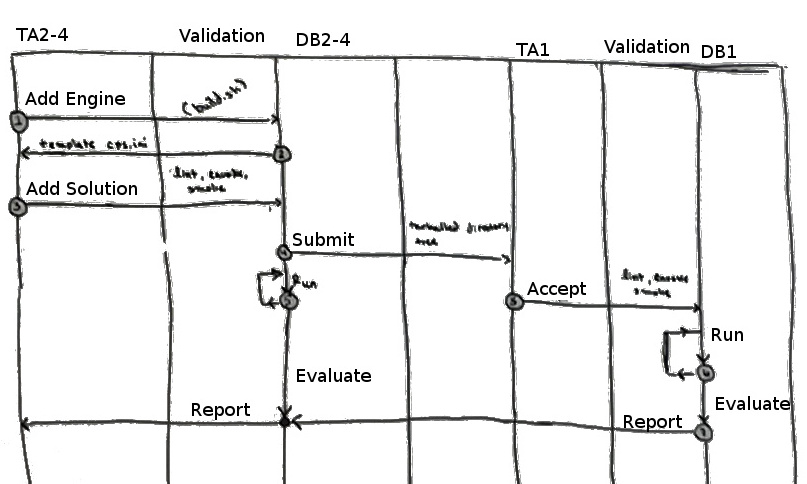
\includegraphics[width=0.9\textwidth]{sequence_diagram.jpg}
  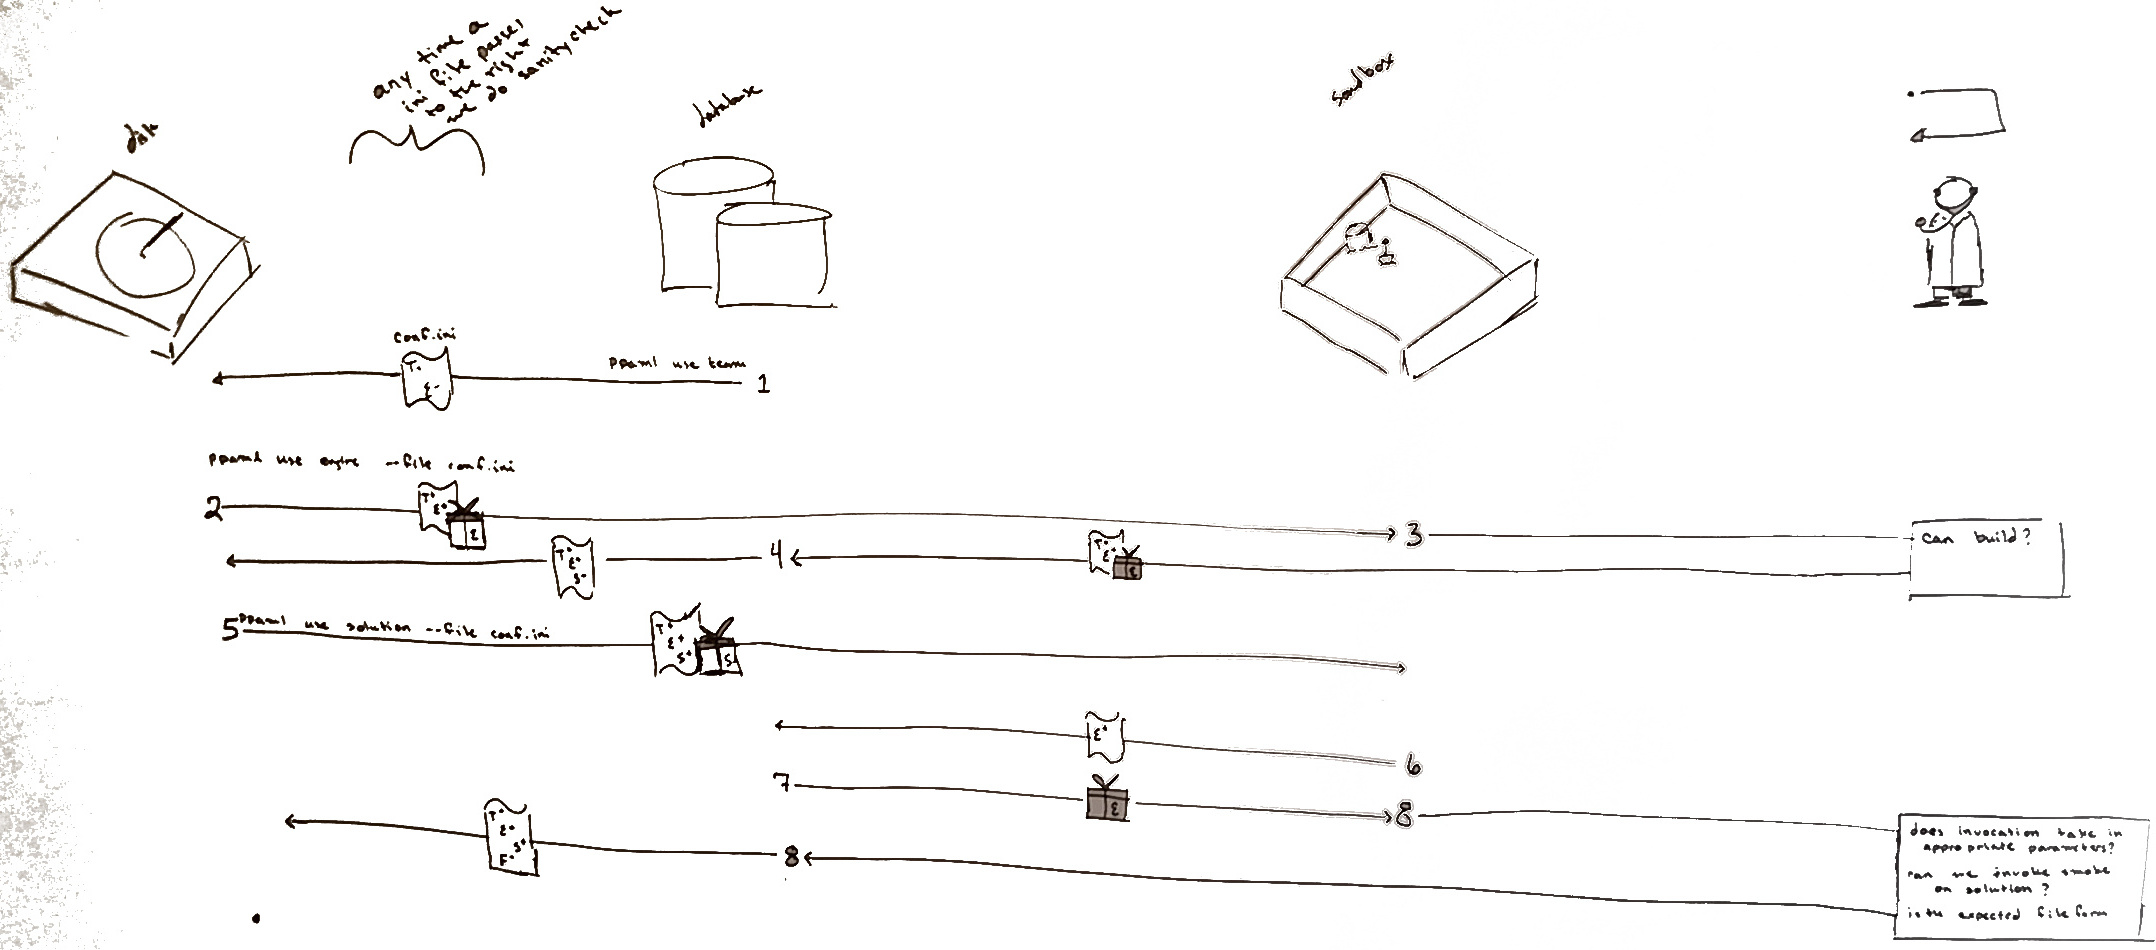
\includegraphics[width=0.9\textwidth]{more_sequence.jpg}
  \end{center}


\end{document}
